\section{Ejercicio 6}
\subsection{Introducción}

Se implementó una ALU con las siguientes operaciones: suma, resta, complemento a dos, shift left, y como operaciones bit a bit: AND, OR, NOT, XOR.
Se tomó como entrada dos nibbles como los operandos, y un selector de 3 bits para seleccionar la operación. Por el otro lado, la salida consta de un resultado, además de un bit de carry u overflow.
Se reutilizaron la mayor cantidad posible de módulos previamente programados y testeados en los incisos anteriores. La razón de esto es que si se testearon los módulos de manera individual, al combinarlos, no habrá que volver a probarlos, pues ya han sido testeados. Es decir, asegurándonos que cada módulo funciona individualmente, la combinación lineal de éstos también funciona, por linealidad.

\subsection{Esquema lógico}
El circuito lógico resultante se presenta a continuación:
\begin{figure}[H]
    \begin{center}
        \caption{Esquema lógico de la ALU.}
		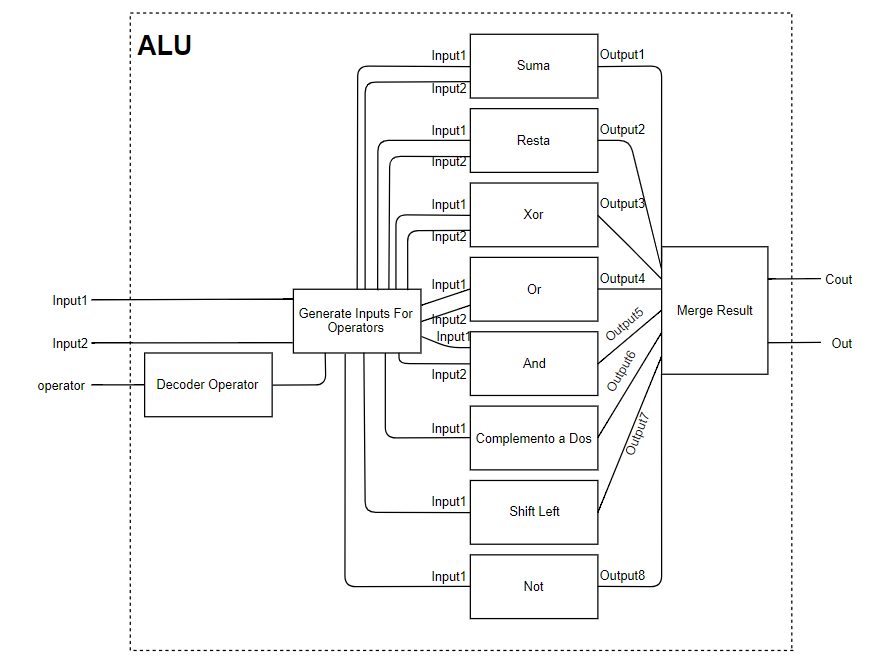
\includegraphics[scale=0.75]{esquemaALU.png}    
	\end{center}
\end{figure}
